% Model-based experimental design: fairness x early-lead, orthogonalised.
% Compile: pdflatex fig_experiment.tex
\documentclass[border=6pt]{standalone}
\usepackage{amsmath,amssymb}
\usepackage{tikz}
\usetikzlibrary{arrows.meta,positioning,fit,calc}
\definecolor{leg}{HTML}{2A7A36}
\definecolor{ill}{HTML}{6A51A3}
\definecolor{def}{HTML}{B2182B}
\begin{document}
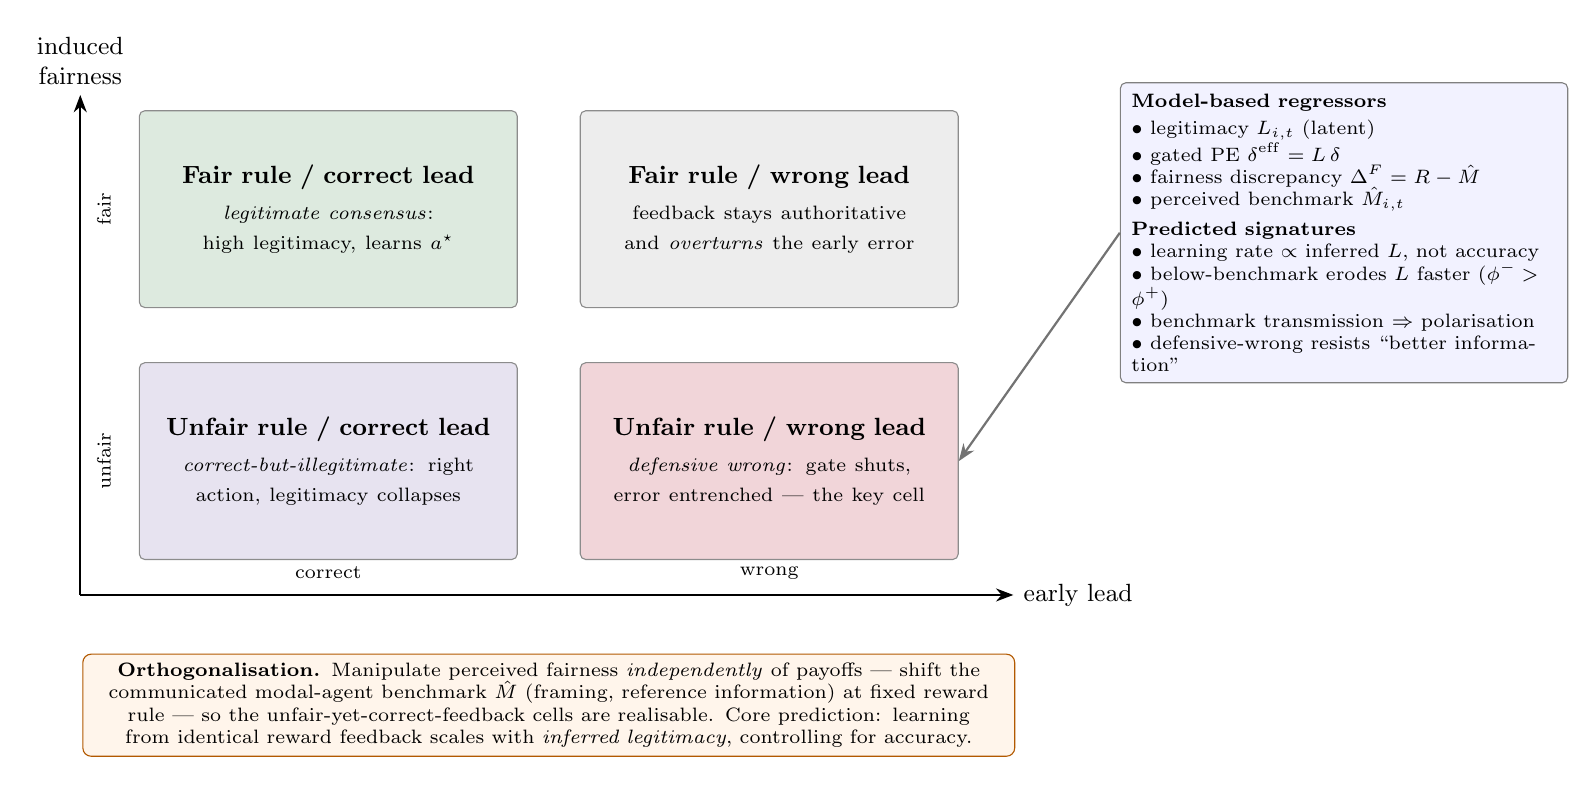
\begin{tikzpicture}[
  font=\small,>={Stealth[length=2.2mm]},
  cell/.style={minimum width=48mm,minimum height=25mm,align=center,
               draw=black!45,rounded corners=2pt,text width=44mm,inner sep=3pt},
  reg/.style={draw=black!50,rounded corners=2pt,fill=blue!5,align=left,
              text width=54mm,inner sep=4pt,font=\scriptsize},
]
% ---- 2x2 design (x: early lead ; y: induced fairness) ------------------
\node[cell,fill=leg!16] (FC) at (0,0)
   {\textbf{Fair rule / correct lead}\\[2pt]\scriptsize \emph{legitimate consensus}:
    high legitimacy, learns $a^\star$};
\node[cell,fill=black!7] (FW) at (5.6,0)
   {\textbf{Fair rule / wrong lead}\\[2pt]\scriptsize feedback stays authoritative
    and \emph{overturns} the early error};
\node[cell,fill=ill!16] (UC) at (0,-3.2)
   {\textbf{Unfair rule / correct lead}\\[2pt]\scriptsize \emph{correct-but-illegitimate}:
    right action, legitimacy collapses};
\node[cell,fill=def!18] (UW) at (5.6,-3.2)
   {\textbf{Unfair rule / wrong lead}\\[2pt]\scriptsize \emph{defensive wrong}: gate
    shuts, error entrenched --- the key cell};
% axes
\draw[->,thick] (-3.15,-4.9) -- (-3.15,1.45) node[above,align=center]{induced\\fairness};
\node[rotate=90,font=\scriptsize] at (-2.85,0){fair};
\node[rotate=90,font=\scriptsize] at (-2.85,-3.2){unfair};
\draw[->,thick] (-3.15,-4.9) -- (8.7,-4.9) node[right,align=center]{early lead};
\node[font=\scriptsize] at (0,-4.62){correct};
\node[font=\scriptsize] at (5.6,-4.62){wrong};

% ---- orthogonalisation note -------------------------------------------
\node[draw=orange!70!black,rounded corners=3pt,fill=orange!8,text width=116mm,
      align=center,font=\scriptsize] (OR) at (2.8,-6.3)
  {\textbf{Orthogonalisation.} Manipulate perceived fairness \emph{independently}
   of payoffs --- shift the communicated modal-agent benchmark $\hat M$ (framing,
   reference information) at fixed reward rule --- so the unfair-yet-correct-feedback
   cells are realisable. Core prediction: learning from identical reward feedback
   scales with \emph{inferred legitimacy}, controlling for accuracy.};

% ---- model-derived regressors -----------------------------------------
\node[reg] (RG) at (12.9,-0.3)
  {\textbf{Model-based regressors}\\[2pt]
   $\bullet$ legitimacy $L_{i,t}$ (latent)\\
   $\bullet$ gated PE $\delta^{\mathrm{eff}}=L\,\delta$\\
   $\bullet$ fairness discrepancy $\Delta^F=R-\hat M$\\
   $\bullet$ perceived benchmark $\hat M_{i,t}$\\[3pt]
   \textbf{Predicted signatures}\\
   $\bullet$ learning rate $\propto$ inferred $L$, not accuracy\\
   $\bullet$ below-benchmark erodes $L$ faster ($\phi^-\!>\!\phi^+$)\\
   $\bullet$ benchmark transmission $\Rightarrow$ polarisation\\
   $\bullet$ defensive-wrong resists ``better information''};
\draw[->,thick,black!55] (RG.west) -- (UW.east);
\end{tikzpicture}
\end{document}
